%; whizzy chapter
% -initex iniptex -latex platex -format platex -bibtex jbibtex -fmt fmt
% 以上 whizzytex を使用する場合の設定。

%     Kansai Debian Meeting resources
%     Copyright (C) 2007 Takaya Yamashita
%     Thank you for Tokyo Debian Meeting resources

%     This program is free software; you can redistribute it and/or modify
%     it under the terms of the GNU General Public License as published by
%     the Free Software Foundation; either version 2 of the License, or
%     (at your option) any later version.

%     This program is distributed in the hope that it will be useful,
%     but WITHOUT ANY WARRANTY; without even the implied warranty of
%     MERCHANTABILITY or FITNESS FOR A PARTICULAR PURPOSE.  See the
%     GNU General Public License for more details.

%     You should have received a copy of the GNU General Public License
%     along with this program; if not, write to the Free Software
%     Foundation, Inc., 51 Franklin St, Fifth Floor, Boston, MA  02110-1301 USA

%  preview (shell-command (concat "evince " (replace-regexp-in-string "tex$" "pdf"(buffer-file-name)) "&"))
% 画像ファイルを処理するためにはebbを利用してboundingboxを作成。
%(shell-command "cd image200708; ebb *.png")

%%ここからヘッダ開始。

\documentclass[mingoth,a4paper]{jsarticle}
\usepackage{kansaimonthlyreport}
\usepackage[dvips]{xy}


% 日付を定義する、毎月変わります。
\newcommand{\debmtgyear}{2009}
\newcommand{\debmtgdate}{23}
\newcommand{\debmtgmonth}{8}
\newcommand{\debmtgnumber}{26}

\begin{document}

\begin{titlepage}

% 毎月変更する部分、本文の末尾も修正することをわすれずに

 第\debmtgnumber{}回 関西 Debian 勉強会資料

\vspace{2cm}

\begin{center}
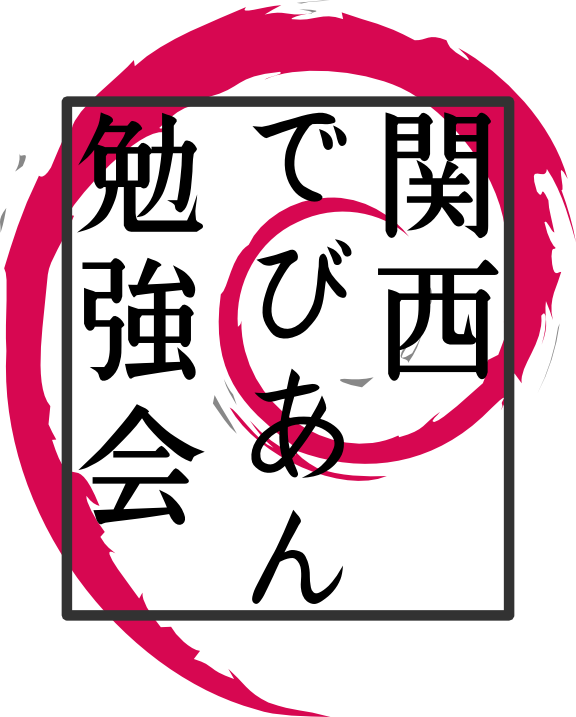
\includegraphics{image200802/kansaidebianlogo.png}
\end{center}

\begin{flushright}
\hfill{}関西 Debian 勉強会担当 のがた・倉敷\\
\hfill{}\debmtgyear{}年\debmtgmonth{}月\debmtgdate{}日
\end{flushright}

\thispagestyle{empty}
\end{titlepage}

\dancersection{Introduction}{Debian JP}
 
 関西 Debian 勉強会はDebian GNU/Linux のさまざ
 まなトピック(新しいパッケージ、Debian 特有の機能の仕組、Debian 界隈で起
 こった出来事、などなど)について話し合う会です。

 目的として次の三つを考えています。
 \begin{itemize}
  \item MLや掲示板ではなく、直接顔を合わせる事での情報交換の促進
  \item 定期的に集まれる場所
  \item 資料の作成
 \end{itemize}

 それでは、楽しい一時をお楽しみ下さい。

\newpage

\begin{minipage}[b]{0.2\hsize}
 {\rotatebox{90}{\fontsize{80}{80}
{\gt 関西デビアン勉強会}}}
\end{minipage}
\begin{minipage}[b]{0.8\hsize}
\hrule
\vspace{2mm}
\hrule
\setcounter{tocdepth}{1}
\tableofcontents
\vspace{2mm}
\hrule
\end{minipage}

%-------------------------------
\dancersection{最近のDebian関係のイベント報告}{のがたじゅん}

こんにちは。のがたじゅんです。
7月におこなわれたDebian関係のイベントについて報告します。

\subsection{オープンソースカンファレンス 2009 Kyoto}

オープンソースカンファレンス 2009 Kyotoが、7月10日と11日京都コンピュータ
学院京都駅前校にて開催され、関西Debian勉強会も参加しました。

\subsubsection{展示ブース}

 \begin{wrapfigure}{l}{7cm}
  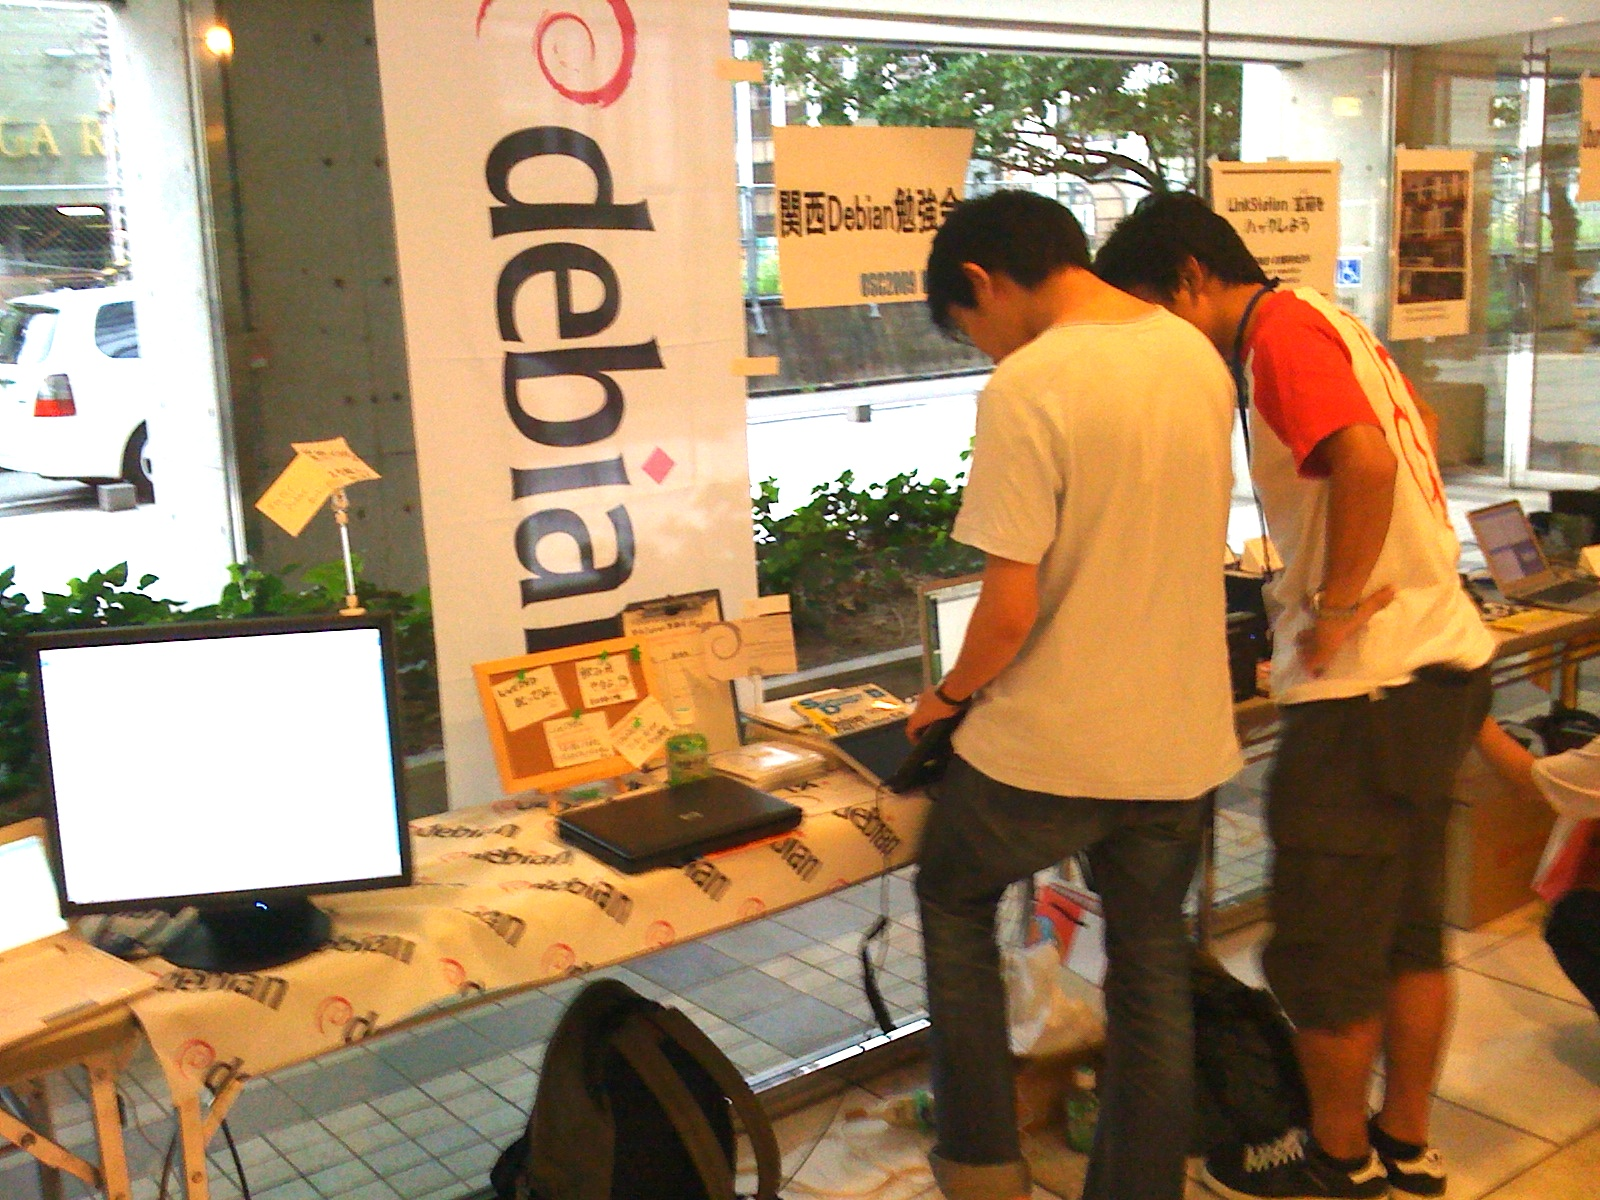
\includegraphics[width=7cm]{image200908/kansai-event-osc2009.jpg}
 \end{wrapfigure}

ブースは10日、11日両日に出展しました。
展示内容は、SDカードにDebian Liveを入れたeeePCとDebian GNU/kFreeBSDをイン
ストールしたDELL Inspiron mini 9の展示。 Tシャツと「あんどきゅめん
てっどでびあん」の販売、Debian Live DVDの配布をおこないました。

今年は例年になく好評で、販売物や配布物が予想より早くなくなったり、来場さ
れた方のなかに、sidを使って野良パッケージも作っているという高校生や、熱心
に質問される女性の方などいらっしゃって、今後も勉強会に参加してほしいなと
思うかたがいました。

展示物では、Debian GNU/kFreeBSDが普段LinuxやBSDを使っている人には違いがす
ぐに理解してもらえ、とてもウケていたのですが、使っていない人にとってはご
く自然に動いているように見えて、何が面白いのかサッパリわからないという困っ
た状況がありました。これからはこの面白さを伝えられるようにしたいですね。

\subsubsection{セッション}
セッションは「DebianとDebian GNU/kFreeBSDの紹介」と題して、第25回関西
Debian勉強会を開催しました。

セッション前半は倉敷さんに「Debianの紹介」ということで、Debian Projectや
Debian JP Projectがどういったことをしているのかや、関西Debian勉強会につい
て紹介していただきました。技術的な面だけでなく、ドキュメントの翻訳など技
術的なこと以外でもProjectに参加できることがわかって、よかったですね。

セッション後半は、大浦さんに「Debian GNU/kFreeBSDの紹介」というタイトル
で、Debian GNU/kFreeBSDの紹介をしていただきました。Debian
GNU/kFreeBSDは、Linuxアーキテキクチャ以外で初めてサポートされたDebianとい
うことで、参加された人の関心もとても高かったようでした。

セッションに参加された人数は数えていませんでしたが、定員50人の教室が一
杯、若干の立ち見も出たので、かなり大盛況だったのではないでしょうか。

\subsection{DebConf9}
Debian開発者が一同に会するカンファレンス、DebConf 9が7月23日から30日まで
スペインのエストレマドゥーラ州カセレス市で行われました。
その様子がビデオで公開されているので、ご覧になってはいかがでしょうか。
\footnote{DebConf9/Streams - Wiki \url{http://wiki.debconf.org/wiki/DebConf9/Streams}}
\footnote{Index of /pub/debian-meetings/2009/debconf9 \url{http://ftp.acc.umu.se/pub/debian-meetings/2009/debconf9/}}

また、日本から参加された 4 名の方が、参加レポートを東京の勉強会資料に寄稿されています。
\footnote{第55回東京エリアDebian勉強会 \url{http://tokyodebian.alioth.debian.org/2009-08.html}}

\subsection{オープンフォース Debian勉強会 徳島}
鳴門のうず潮はDebianのぐるぐる。
ということで、8月7日徳島シビックホールで開催された、
「オープンフォース Debian勉強会 徳島」に参加してきました。

この勉強会はDebian Users MLで河野@南部製作所さんが呼びかけて始まった、徳
島のDebianユーザー有志で行う勉強会ということで、楽しみにしていたのです
が、徳島市内に入ったところで高速バスが帰宅ラッシュに巻き込まれ、会場の付
近にもかかわらず、まったく動くことができない事態発生。
そうこうしてるうちに時間は過ぎ、会場に着いたのは勉強会が始まってしばらく
経ってからでした。

河野さんが発表された、Debianを使った病院のビデオ上映システム「ビデオ上映
コントローラwvss」についてはあまり聞けませんでしたが、奥さんのみーまさん
が発表された「メシマズ嫁が作るDebianスイーツ(w」は衝撃のDebianの出会い告
白と、その後に出されたぐるぐるをイメージして作られたお手製ロールケーキは
とてもおいしゅうございました。

その後は勉強会を続けていくにあたってのキックオフ会議でしたが、参加された
方は学生の方が多く、活発な意見も多く聞かれ、これからが楽しみな勉強会でし
た。

「オープンフォース Debian勉強会 徳島」はオープンソース系勉強会と交互に隔
月(次回は10月)開催されるそうなので、遊びに行くのもいいのではないでしょう
か。

\begin{figure}[h]
 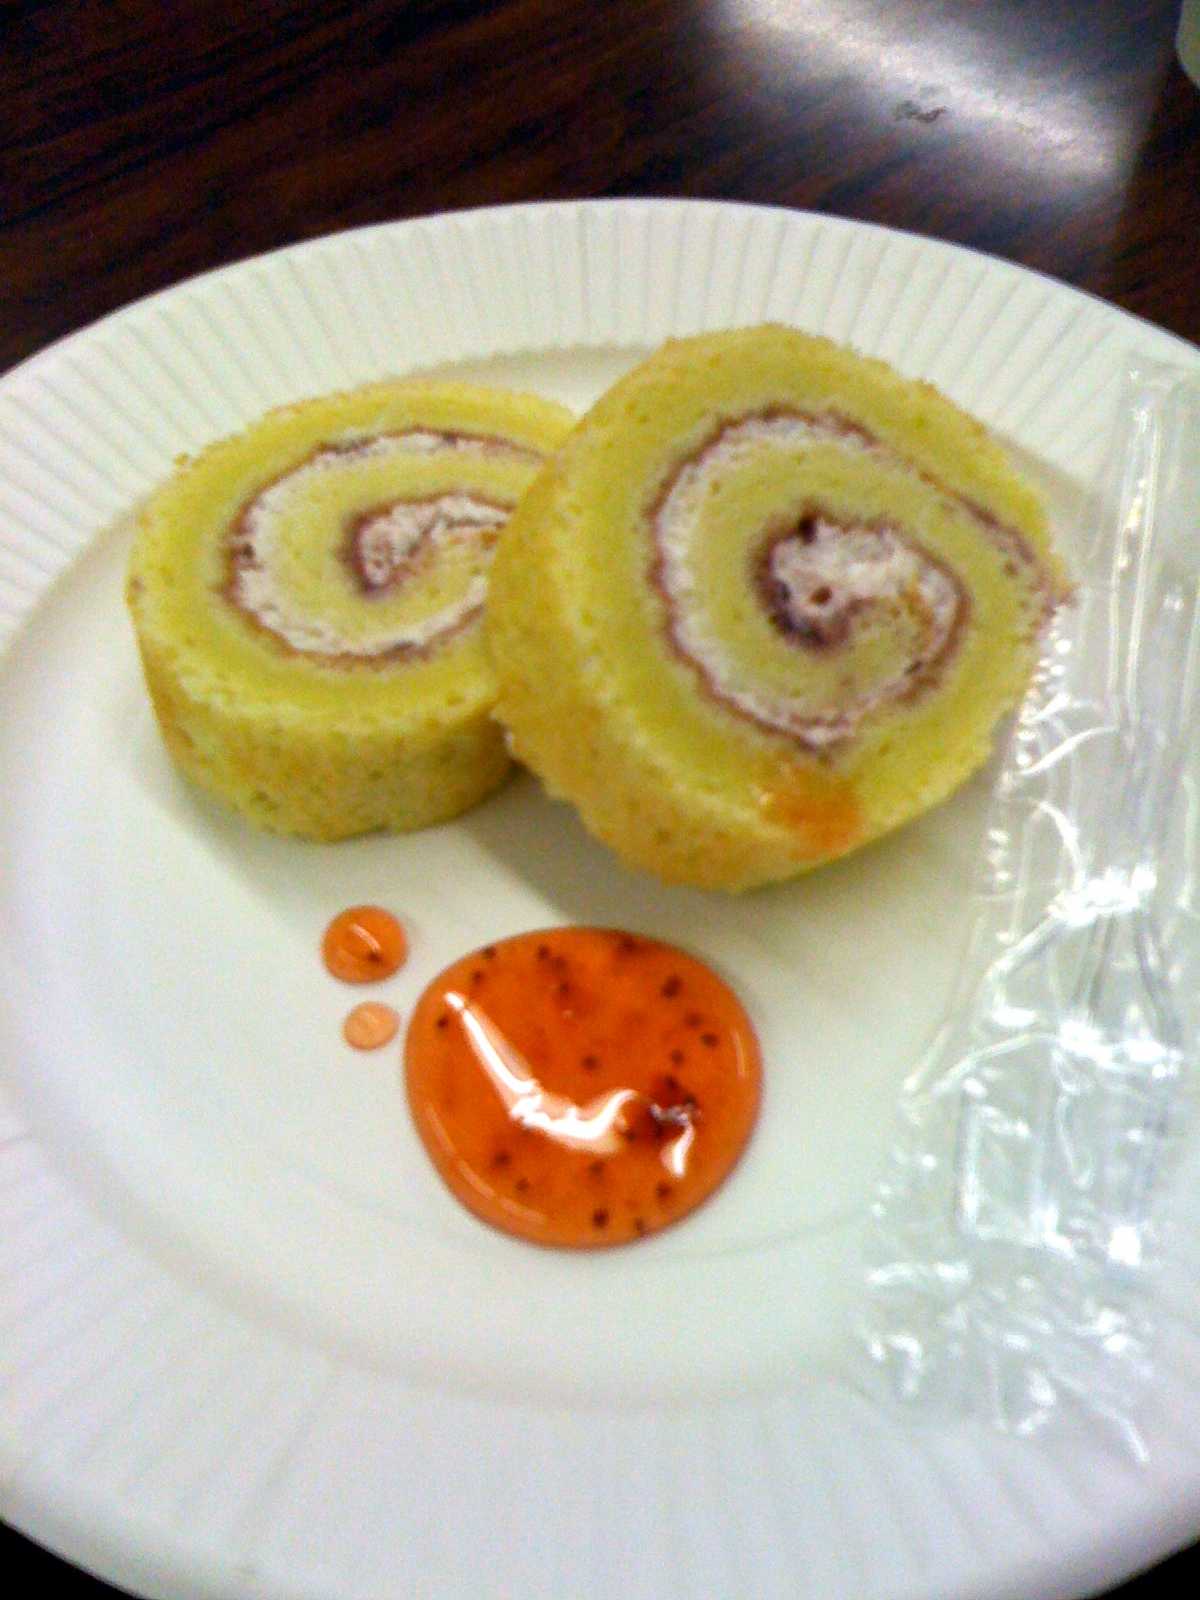
\includegraphics[width=4cm]{image200908/kansai-event-tokushima01.jpg}
 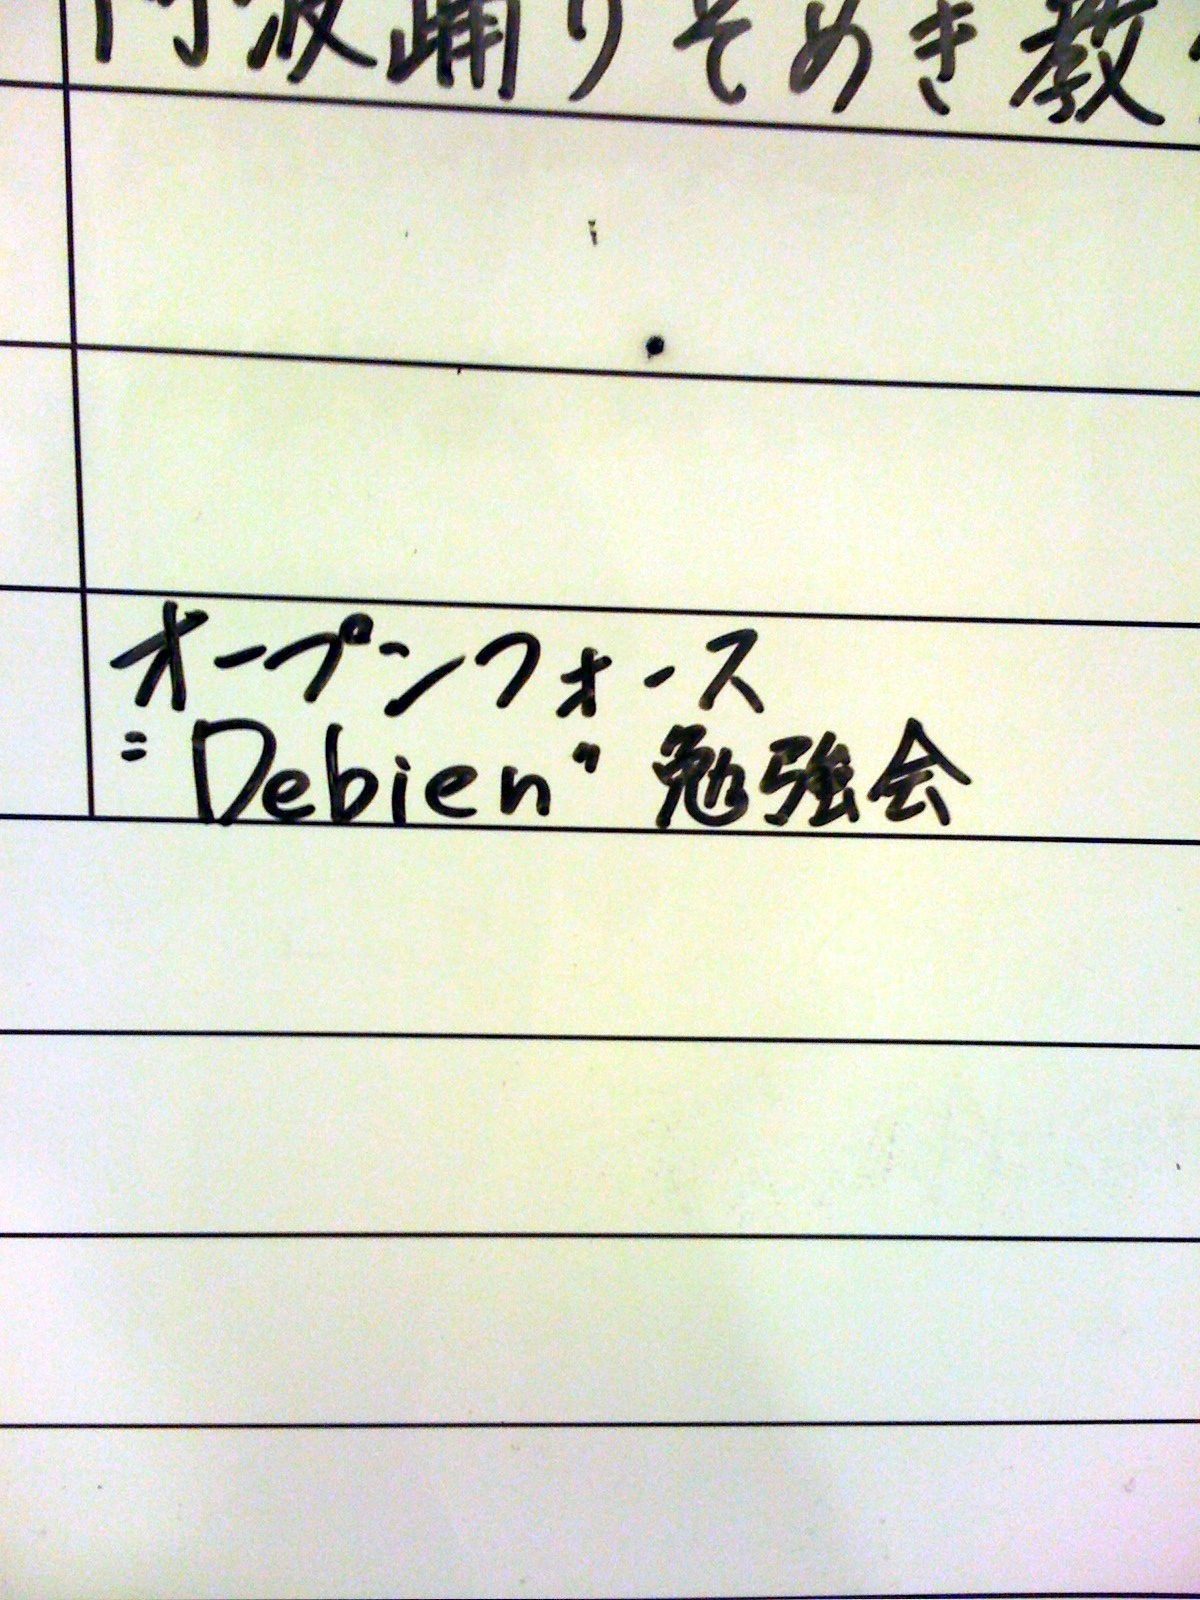
\includegraphics[width=4cm]{image200908/kansai-event-tokushima00.jpg}
\caption{ぐるぐるロールケーキと徳島ではまだまだと思い知らされた掲示板}
\end{figure}

%-------------------------------
\dancersection{DDTSS を使ってみよう}{倉敷 悟}

\subsection{そもそも DDTSS って何?}

シンプルに言うと、「パッケージ説明文」を翻訳するための Web インターフェイスのことです。

解説資料としては、第53回東京エリアDebian勉強会の資料
(\url{http://tokyodebian.alioth.debian.org/2009-06.html})でまとめられています。
今回は、この資料を参照しながら、ハンズオンとして実際に DDTSS を使った翻訳作業をやっていきます。

\subsection{事前課題の確認}

今回は、準備として事前課題の形をとってみましたが、いかがでしたでしょうか。

今後のセッションでも、適宜事前課題をからめていきたいと思っていますので、気づいたことがあれば教えてください。

\subsubsection{DDTSS アカウントの作成}

DDTSS はウェブサービスで、ユーザのアカウントを独自に保持しています。
作業内容や実績はアカウントとひもづけて保管されるので、最初に作っておきましょう。\footnote{DDTSS create login \url{https://ddtp.debian.net/ddtss/index.cgi/createlogin}}
ユーザ ID として利用される、メールアドレスが必要になります。

では作成したアカウントで、DDTSS にログインしてみてください。作成がまだの人はここで作ってしまいましょう。

\subsubsection{気になるパッケージを探す}

DDTSS の翻訳で扱う「パッケージの説明文」は、個別にはあまり量もないですし、翻訳作業をするにあたって、とっかかりの敷居は低い方だと思います。

とはいえ、見たことも聞いたこともないパッケージの説明というのもやっぱり辛いものがありますので、まずは関心があるとか、使っているとか、見たことある、といったものから手をつけてみるといいでしょう。

\subsection{レビューをしてみる}

DDTSS では、誰かが訳した一つの説明文は、オフィシャルの配布データにとりこまれるまでに、3 人からレビューを受けて「修正なしで OK」とされる必要があります。

レビュー 3 人というのは、実は結構高いハードルで、ついついレビュー待ちのものがたまってしまいがちです。

そういうわけで、いきなり翻訳するというのはしんどいなぁ、という方も、ひとまずレビューにチャレンジしてみましょう。
すでに翻訳された文章を確認するだけなので、敷居は低いと思います。

この文章を書いている時点では、レビュー待ちの数がずいぶん少ないので、選ぶのに困ってしまうかも知れませんが……。

\subsubsection{レビュー待ち一覧の見方}

DDTSS のログイン画面を、下の方にスクロールしてみてください。
「Pendingreview」と書かれたセクションがあるはずです。
下に並んでいるパッケージが、レビューを待っているもので、「Pending review」の横にある数字はその合計数になります。各パッケージ名の横を見ると、レビューの状況がわかります。

「needs initial review」は、翻訳された後まだ一回もレビューされていないということです。

「needs review had x」は、レビュー途上にあるもので、x がレビューされた回数を示しています。

\subsubsection{レビュー画面}

ではパッケージを選んでみましょう。レビュー画面に切り替わります。
いくつかのメタ情報と合わせて、パッケージの説明文が、原文と対比される形で表示されているはずです。

まず、訳文を読んでみてください。意味は通りますか?  誤字はありませんか?
おかしいな、と思ったところは、原文と見比べてみてください。

レビューしてみて、特に訂正が必要ない状態であれば、「Accept as is」ボタンを押します。これで、レビューカウントが 1 つ増えることになります。

これはどう見てもおかしいな、というところがあれば、フォームの上で編集して、「Accept with changes」ボタンを押します。
訳文は変更されて、レビューは振り出しに戻ることになります。

ちょっと違う気がするんだけど、いまいち自信がない……という場合は、コメント欄 (comment field) がありますので、そこに書いて、「Change comment only」ボタンを押します。この場合、レビューとしては何も変更されず、コメントだけ追記されることになります。

開いてみたけど、やっぱりレビューをやめる、という場合は、何もボタンを押さずに戻ってください。

\subsubsection{実際にレビューしてみる}

少しまとまった時間をとりますので、レビューにチャレンジしてみてください。
わからないことがあれば、適宜呼んでください。

\subsection{最初の翻訳文作成}

いくつかレビューをしてみて DDTSS にも慣れてきたら、翻訳にも手を出してみてください。
翻訳されていないパッケージ説明文は、「Pending Translation」の一覧にあります。気になるものを選んでみましょう。

画面の構成は、レビューとほとんど同じですが、翻訳文は、あったりなかったりします。
翻訳文がある場合でも、原文が更新されていたり、似ている別のパッケージからひっぱられたりしているので、何らかの修正は必要になるはずです。

実際の翻訳画面にも赤字で表示されますが、やっぱり翻訳をやめる、という場合には「Abandon」というボタンを押すことになっているので注意してください。

ここは、時間が許せば実際にやってみようと思います。

%-------------------------------
\dancersection{lintian でパッケージをチェックする}{大浦 真}

\subsection{lintianとは}

\begin{itemize}
\item Debian パッケージには、さまざまなポリシーや作法が存在し、
  主に以下の文書にまとまっている。
  \begin{itemize}
  \item Debianポリシーマニュアル
    (\url{http://www.debian.org/doc/debian-policy/})
  \item Debian 開発者リファレンス
    (\url{http://www.debian.org/doc/developers-reference/})
  \end{itemize}
\item これらの内容を全て手動でチェックするのは困難なので、チェックするために
  \textbf{lintian} というツールが存在する。
\item パッケージがポリシーに合致しているかどうかを
  ある程度チェックできる。
  (完全に全てチェックできるわけではない。)
\item 元々 C言語で文法をチェックするためのツールとして
  \textbf{lint} というものが存在した。
  \begin{itemize}
  \item lint とは、元々、機織りの際に出る糸くずやほつれ糸を指す。
  \item Debian には、\textbf{splint} というパッケージが存在する。
  \item C言語以外でも文法チェックのツールの名前としてよく使われる。
    \url{http://openlab.ring.gr.jp/k16/htmllint/} (Another HTML-lint) など。
  \end{itemize}
\item lintian は 1998年に開発が始まった。perl ベース。
\item 一時期、同様の機能を持った \textbf{linda} というツールもあったが
  こちらは lenny から削除された。
\end{itemize}

\subsection{lintianの使い方}

\begin{itemize}
\item 完成したバイナリパッケージ(\texttt{.deb})と
  ソースパッケージ(\texttt{.dsc})に対してチェックを行う。
\item \textbf{debuild}でパッケージをビルドすると
  ビルド後に自動的に \texttt{lintian} が実行される。
\item 手動でチェックする場合は、\texttt{lintian} コマンドの引数に
  \texttt{.changes} ファイルを
  指定すると、バイナリパッケージとソースパッケージを同時にチェックできる。
  (\texttt{.changes} の中には、バイナリパッケージとソースパッケージの
  ファイル名が書かれている。)
  \begin{description}
  \item[-c] 通常のチェックを行う。(省略可)
  \item[-i] 詳しい説明も同時に表示する。
  \item[-I] 付加的な内容のチェックも行う。
  \end{description}
\end{itemize}

\subsection{具体例}


\subsubsection{hello-debhelper の場合}

\begin{itemize}
\item 以下では、\textbf{hello-debhelper}(2.4-1)をサンプルとして説明する。
  (\textbf{lintian} のバージョンは 2.2.14。)
\item オプションなしで \texttt{.changes} ファイルを
  指定して \texttt{lintian} を実行
  \begin{screen}[5]
    {\footnotesize{}
\begin{verbatim}
% lintian hello-debhelper_2.4-1_amd64.changes
E: hello-debhelper: package-contains-info-dir-file usr/share/info/dir.gz
W: hello-debhelper: install-info-used-in-maintainer-script prerm:3
W: hello-debhelper: install-info-used-in-maintainer-script postinst:4
W: hello-debhelper: missing-dependency-on-install-info
\end{verbatim}
    }
  \end{screen}
\item `E: 'から始まるものはエラー、`W: ' から始まるものは警告。
\item 詳しい内容は -i オプションで見ることができる。
  \begin{screen}[5]
    {\footnotesize{}
\begin{verbatim}
% lintian -i hello-debhelper_2.4-1_amd64.changes
E: hello-debhelper: package-contains-info-dir-file usr/share/info/dir.gz
N: 
N:    This package contains a file named dir or dir.old, possibly compressed,
N:    in /usr/share/info. This is the directory (or backup) of info pages and
N:    is generated automatically by install-info when a package containing
N:    info documentation is installed. Some upstream build systems create it
N:    automatically, but it must not be included in a package since it needs
N:    to be generated dynamically based on the installed info files on the
N:    system.
N:    
N:    Severity: important, Certainty: certain
N: 
W: hello-debhelper: install-info-used-in-maintainer-script prerm:3
N: 
N:    This script apparently runs install-info. Updating the
N:    /usr/share/info/dir file is now handled automatically by triggers, so
N:    running install-info from maintainer scripts is no longer necessary.
N:    
N:    If debhelper generated the maintainer script fragment, rebuilding the
N:    package with debhelper 7.2.17 or later will fix this problem.
N:    
N:    Severity: normal, Certainty: possible
N: 
W: hello-debhelper: install-info-used-in-maintainer-script postinst:4
W: hello-debhelper: missing-dependency-on-install-info
N: 
N:    This package appears to contain at least one info document but does not
N:    depend on dpkg (>= 1.15.4) | install-info as recommended by Policy. This
N:    dependency is needed for the transition to triggerized install-info to
N:    correctly build the info directory during partial upgrades from lenny.
N:    
N:    Refer to Debian Policy Manual section 12.2 (Info documents) for details.
N:    
N:    Severity: normal, Certainty: possible
N: 
\end{verbatim}
    }
  \end{screen}
\item 一つ目のエラー: 「パッケージの中に usr/share/info/dir.gz が
  含まれている。」
  \begin{itemize}
  \item info ディレクトリの中の dir ファイルは info の目次に相当するもので、
    Debian では、\texttt{install-info} コマンドで自動的に作られるものなので、
    パッケージに含めるべきではない。
  \item \texttt{debian/rules} の install ターゲットの中で
    dir ファイルを削除する。
  \end{itemize}
\item 二つ目、三つ目の警告: 「install-info コマンドが postint と prerm の
  中で実行されている。」
  \begin{itemize}
  \item \texttt{install-info} コマンドは、
    dpkg の trigger という機能で自動的に
    実行されるので、postinst と prerm で実行する必要はない。
  \item \texttt{debian/postinst} と \texttt{debian/prerm} を削除。
    (このパッケージでは、他に postinst、prerm を使っていないので、
    \texttt{install-info}コマンドの部分だけを消すと、
    「postinst、prerm が空っぽだ」という警告が出る。)
  \end{itemize}
\item 四つ目の警告: 「install-info への依存がない。」
  \begin{itemize}
  \item \texttt{install-info} コマンドが入っている
    \textbf{install-info} パッケージに対する依存関係がない。
    Debian ポリシー 12.2 参照。

    \url{http://www.debian.org/doc/debian-policy/ch-docs.html#s12.2}
  \item debian/control に `\verb:dpkg (>= 1.15.4) | install-info:' と
    追加する。
  \end{itemize}
\item これで `lintian clean' になる。
\end{itemize}

\subsubsection{よくある警告}

\begin{itemize}
\item よく見かける警告
  \begin{screen}[5]
  {\footnotesize{}
\begin{verbatim}
W: hello-debhelper source: out-of-date-standards-version 3.8.0 (current is 3.8.3)
W: hello-debhelper: binary-without-manpage usr/bin/hello2
\end{verbatim}
    }
  \end{screen}
  \begin{screen}[5]
    {\footnotesize{}
\begin{verbatim}
W: hello-debhelper source: out-of-date-standards-version 3.8.0 (current is 3.8.3)
N: 
N:    The source package refers to a Standards-Version older than the one that
N:    was current at the time the package was created (according to the
N:    timestamp of the latest debian/changelog entry). Please consider
N:    updating the package to current Policy and setting this control field
N:    appropriately.
N:    
N:    If the package is already compliant with the current standards, you
N:    don't have to re-upload the package just to adjust the Standards-Version
N:    control field. However, please remember to update this field next time
N:    you upload the package.
N:    
N:    See /usr/share/doc/debian-policy/upgrading-checklist.txt.gz in the
N:    debian-policy package for a summary of changes in newer versions of
N:    Policy.
N:    
N:    Severity: normal, Certainty: certain
N: 
W: hello-debhelper: binary-without-manpage usr/bin/hello2
N: 
N:    Each binary in /usr/bin, /usr/sbin, /bin, /sbin or /usr/games should
N:    have a manual page
N:    
N:    Note that though the man program has the capability to check for several
N:    program names in the NAMES section, each of these programs should have
N:    its own manual page (a symbolic link to the appropriate manual page is
N:    sufficient) because other manual page viewers such as xman or tkman
N:    don't support this.
N:    
N:    If the name of the man page differs from the binary by case, man may be
N:    able to find it anyway; however, it is still best practice to make the
N:    case of the man page match the case of the binary.
N:    
N:    If the man pages are provided by another package on which this package
N:    depends, lintian may not be able to determine that man pages are
N:    available. In this case, after confirming that all binaries do have man
N:    pages after this package and its dependencies are installed, please add
N:    a lintian override.
N:    
N:    Refer to Debian Policy Manual section 12.1 (Manual pages) for details.
N:    
N:    Severity: normal, Certainty: possible
\end{verbatim}
      }
  \end{screen}
\item 一つ目の警告: 「Standards-Version が古い。」
  \begin{itemize}
  \item Debian ポリシー、および、それに付随する文書のバージョンを
    Standards-Version と呼ぶ。
    debian-policy パッケージのバージョン番号で、現時点での最新版は
    3.8.3.0 である。
    パッケージは、どの Standards-Version に従っているか debian/control で
    指定するが、古すぎると警告が出る。
  \item debian-policy パッケージの中の upgrading-checklist.txt で変更点を
    確認し、パッケージを更新する。
  \end{itemize}
\item 二つ目の警告: 「マニュアルページがない。」
  \begin{itemize}
  \item /usr/bin、/usr/sbin、/bin、/sbin などにあるバイナリに対して
    マニュアルページがない。
    Debian としては、コマンドに対するマニュアルページは必須になる。
    Debian ポリシー 12.1 参照。
  \item 上流のソースにマニュアルページがあればそれをインストールし、
    なければ自分で作成する。
  \end{itemize}
\end{itemize}

\subsection{まとめ}

\begin{itemize}
\item lintian はスクリプトでパッケージをチェックするだけなので、
  ポリシーの全ての内容を確認することはできない。
  必要に応じてポリシーを自分で確認する必要がある。
\item 事情により、どうしてもチェックを外したい時は、overrides を使うことが
  できる。(/usr/share/lintian/overrides/ 参照)
  \begin{itemize}
  \item /usr/share/lintian/overrides/adduser の内容
  \end{itemize}
  \begin{screen}[5]
    {\footnotesize{}
\begin{verbatim}
adduser: maintainer-script-needs-depends-on-adduser postinst
adduser: maintainer-script-needs-depends-on-adduser postrm
adduser: maintainer-script-needs-depends-on-adduser config
\end{verbatim}
      }
  \end{screen}
\item チェックの内容を調べることにより、パッケージングシステムの
  仕組みを深く知ることができる。
\end{itemize}

%-------------------------------
\dancersection{今後の予定}{倉敷 悟}

\subsection{次回}
次回は、2009年09月27日に京都リサーチパークで行います。初めての会場となりますので、ご注意ください。

% 冊子にするために、4の倍数にする必要がある。
% そのための調整
% \dancersection{メモ}{}
% \mbox{}\newpage
% \mbox{}\newpage

\printindex
 \cleartooddpage

 \begin{minipage}[b]{0.2\hsize}
  \rotatebox{90}{\fontsize{80}{80} {\gt 関西デビアン勉強会} }
 \end{minipage}
 \begin{minipage}[b]{0.8\hsize}

 \vspace*{15cm}
 \rule{\hsize}{1mm}
 \vspace{2mm}
 
\includegraphics[width=2cm]{image200502/openlogo-nd.eps}
 \noindent \Large \bf Debian 勉強会資料\\ \\
 \noindent \normalfont \debmtgyear{}年\debmtgmonth{}月\debmtgdate{}日 \hspace{5mm}  初版第1刷発行\\
 \noindent \normalfont 関西 Debian 勉強会 (編集・印刷・発行)\\
 \rule{\hsize}{1mm}
 \end{minipage}

\end{document}
